\documentclass{article}
\usepackage[preprint]{neurips_2023}
\usepackage{amsmath,amssymb}
\usepackage{graphicx}
\usepackage{booktabs}
\usepackage{hyperref}
\usepackage{placeins}

\title{A Minimal Decision Capacity Threshold Prevents\\Catastrophic Exploitation in Self-Play RL}

\author{
  Arahan Kujur\\
  Independent Researcher\\
  \texttt{kujurarahan@gmail.com}
}

\begin{document}
\maketitle

% ===================================================================
\begin{abstract}
We show that a minimal threshold in decision capacity determines whether self-play reinforcement learning agents collapse under asymmetric rule perturbations. In Kuhn and Leduc Poker, we remove Player~0's ability to bet or raise---either at all decision nodes or only at the opening move. Across five seeds with paired card deals: (i)~complete removal causes adaptive Q-learning to collapse to near-maximal exploitation (Kuhn:~$-0.93$; Leduc:~$-0.31$), while a frozen Q-learning baseline stays near~$-0.14$, confirming the collapse is co-adaptation-driven; (ii)~preserving a single decision point stabilises Q-learning near Nash equilibrium (Kuhn:~$-0.07$; Leduc:~$-0.10$); (iii)~the pattern is timing-invariant: early, mid, and late perturbation produce identical collapse severity; (iv)~collapse is fast, occurring within four episodes on average in Kuhn. These results establish a sharp threshold effect between zero and minimal decision capacity that is game-general, not Kuhn-specific.
\end{abstract}

% ===================================================================
\section{Introduction}

Multi-agent reinforcement learning (MARL) agents trained through self-play have achieved superhuman performance in complex games~\citep{silver2018general}, yet their robustness to structural changes in the environment remains poorly understood. Prior work has focused primarily on stochastic perturbations to observations or rewards, or on opponent modelling under distribution shift, leaving structural changes to the action space relatively unexplored. When the rules of a game change asymmetrically---for instance, when one player loses access to certain actions---how do self-play dynamics respond?

We study this question in two imperfect-information poker games: Kuhn Poker and Leduc Poker. After a training phase of normal self-play, we remove Player~0's ability to bet (Kuhn) or raise (Leduc) at a subset of decision nodes. This creates a controlled perturbation to the action space that reduces the agent's \emph{decision capacity}---the number of information sets at which the agent retains more than one legal action.

Our central finding is a sharp threshold effect. When decision capacity drops to zero (every decision is forced), adaptive Q-learning collapses to near-maximal exploitation through a co-adaptation spiral. When even a single decision point is preserved, Q-learning stabilises near Nash equilibrium. A frozen Q-learning baseline---which stops updating at the perturbation point---does not collapse, isolating continued self-play adaptation as the mechanism rather than the constraint itself.

We further show that the collapse is timing-invariant (identical outcomes whether the perturbation is applied early, mid, or late in training) and replicates across both games, ruling out Kuhn-specific artifacts. Our contributions are:
\begin{itemize}
  \item We identify a sharp decision-capacity threshold governing collapse in self-play RL.
  \item We isolate co-adaptation under constraint as the mechanism via a frozen baseline comparison.
  \item We demonstrate timing-invariant collapse across perturbation schedules.
  \item We replicate the phenomenon across two structurally distinct poker games (Kuhn and Leduc).
\end{itemize}

% ===================================================================
\section{Related Work}

\paragraph{Regret minimisation in games.}
Counterfactual regret minimisation (CFR)~\citep{zinkevich2007regret} is the standard algorithm for computing Nash equilibria in imperfect-information games. Its convergence guarantees in two-player zero-sum settings are well-established, and it has been scaled to large poker variants~\citep{bowling2015heads}. We use CFR as a planning baseline whose frozen strategy represents the best-case response to perturbation without adaptation.

\paragraph{Self-play reinforcement learning.}
Self-play has driven major advances in game-playing agents, from TD-Gammon~\citep{tesauro1994td} through AlphaZero~\citep{silver2018general}. However, self-play dynamics can be unstable: agents may cycle, overfit to their own weaknesses, or fail to generalise~\citep{lanctot2019openspiel}. Our work isolates a specific failure mode---co-adaptation-driven collapse under asymmetric constraint changes---that is distinct from the cyclic instabilities studied in general-sum games.

\paragraph{Robustness in multi-agent RL.}
Prior work on robustness in MARL has focused on adversarial perturbations to observations or rewards~\citep{gleave2020adversarial}, domain randomisation, or opponent modelling under distribution shift. Our setting differs: we perturb the \emph{action space} of one player asymmetrically, eliminating decision points rather than adding noise. This structural perturbation reveals a qualitative threshold effect that continuous perturbations would not produce.

% ===================================================================
\section{Background}

\paragraph{Kuhn Poker.}
A two-player zero-sum game with three cards ($J < Q < K$), two actions (pass, bet), and an ante of~1. The Nash equilibrium value for Player~0 is $-1/18 \approx -0.056$.

\paragraph{Leduc Poker.}
A two-player zero-sum game with six cards ($J, Q, K$ in two suits), three actions (fold, check/call, raise), and two rounds of fixed-limit betting (round~1: raise size~2; round~2: raise size~4; maximum two raises per round). The Nash equilibrium value for Player~0 is approximately $-0.087$. Our from-scratch CFR implementation converges to $-0.0866$ after 5{,}000 iterations, matching the known analytical value.

\paragraph{Agents.}
We evaluate three agent types:
\begin{itemize}
  \item \textbf{CFR}: Counterfactual regret minimisation, trained to Nash equilibrium offline (deterministic full-tree enumeration). The frozen strategy is shared across seeds.
  \item \textbf{Q-Learning}: Tabular, $\varepsilon$-greedy ($\varepsilon = 0.15$), with Monte Carlo terminal updates. Continues learning after perturbation.
  \item \textbf{QL-Frozen}: Identical to Q-Learning during training. At the perturbation point, the Q-table and $\varepsilon$ are frozen (greedy execution only).
\end{itemize}

% ===================================================================
\section{Methodology}

Each experiment runs five seeds, each consisting of 20{,}000 self-play episodes. A perturbation is applied to Player~0 at episode 10{,}000 unless otherwise noted.

\paragraph{Decision capacity.}
We define \emph{decision capacity} as the number of reachable information sets in which the affected agent retains more than one legal action after perturbation. Capacity~0 means every decision is forced; capacity~1 means exactly one information set retains a genuine choice.

\paragraph{RNG design.}
Four independent random number generator streams are derived per seed: (1)~card deals, shared between all agents for paired comparison; (2)~CFR action selection; (3)~Q-Learning action selection; (4)~QL-Frozen action selection. CFR training uses deterministic full-tree enumeration and runs once outside the seed loop.

\paragraph{Statistical analysis.}
We report paired $t$-tests across seeds, bootstrap 95\% confidence intervals (10{,}000 resamples), and Cohen's~$d$ effect sizes. An adaptive burn-in (first 25\% of each phase, capped at 5{,}000/2{,}000 episodes) is excluded for stable estimates. Due to low across-seed variance under paired evaluation, effect sizes are large and should be interpreted qualitatively as indicating direction and reliability rather than as conventional benchmarks.

\paragraph{Time-to-collapse.}
The first episode at which the 200-episode moving average drops below $-0.5$.

% ===================================================================
\section{Experiments}

\subsection{Kuhn Poker: Full Removal (Capacity 0)}

Bet is removed from Player~0 at all decision nodes. Player~0 has zero remaining decisions: forced check, forced fold.

\begin{table}[ht!]
\centering
\caption{Kuhn Poker, full removal (capacity~0). Mean Player~0 reward with 95\% bootstrap CIs across five seeds.}
\label{tab:kuhn-full}
\begin{tabular}{lcccc}
\toprule
Agent & Pre (95\% CI) & Post (95\% CI) & $p$ & $d$ \\
\midrule
CFR        & $-0.053$ {\small$[-0.066, -0.041]$} & $-0.231$ {\small$[-0.235, -0.228]$} & ${<}0.0001$ & $-11.9$ \\
Q-Learning & $-0.035$ {\small$[-0.046, -0.025]$} & $\mathbf{-0.927}$ {\small$[-0.929, -0.925]$} & ${<}0.0001$ & $-66.1$ \\
\bottomrule
\end{tabular}
\end{table}

As shown in Table~\ref{tab:kuhn-full}, Q-Learning collapses to near $-1.0$: the self-play opponent learns that Player~0 always folds and converges to unconditional betting. The $\varepsilon$-floor (0.15) prevents the average from reaching exactly $-1.0$. CFR drops to $-0.23$, bounded because its opponent also plays Nash.

\textbf{Collapse speed.}~Q-Learning collapsed in all five seeds within a mean of four episodes after perturbation.

\begin{figure}[ht!]
\centering
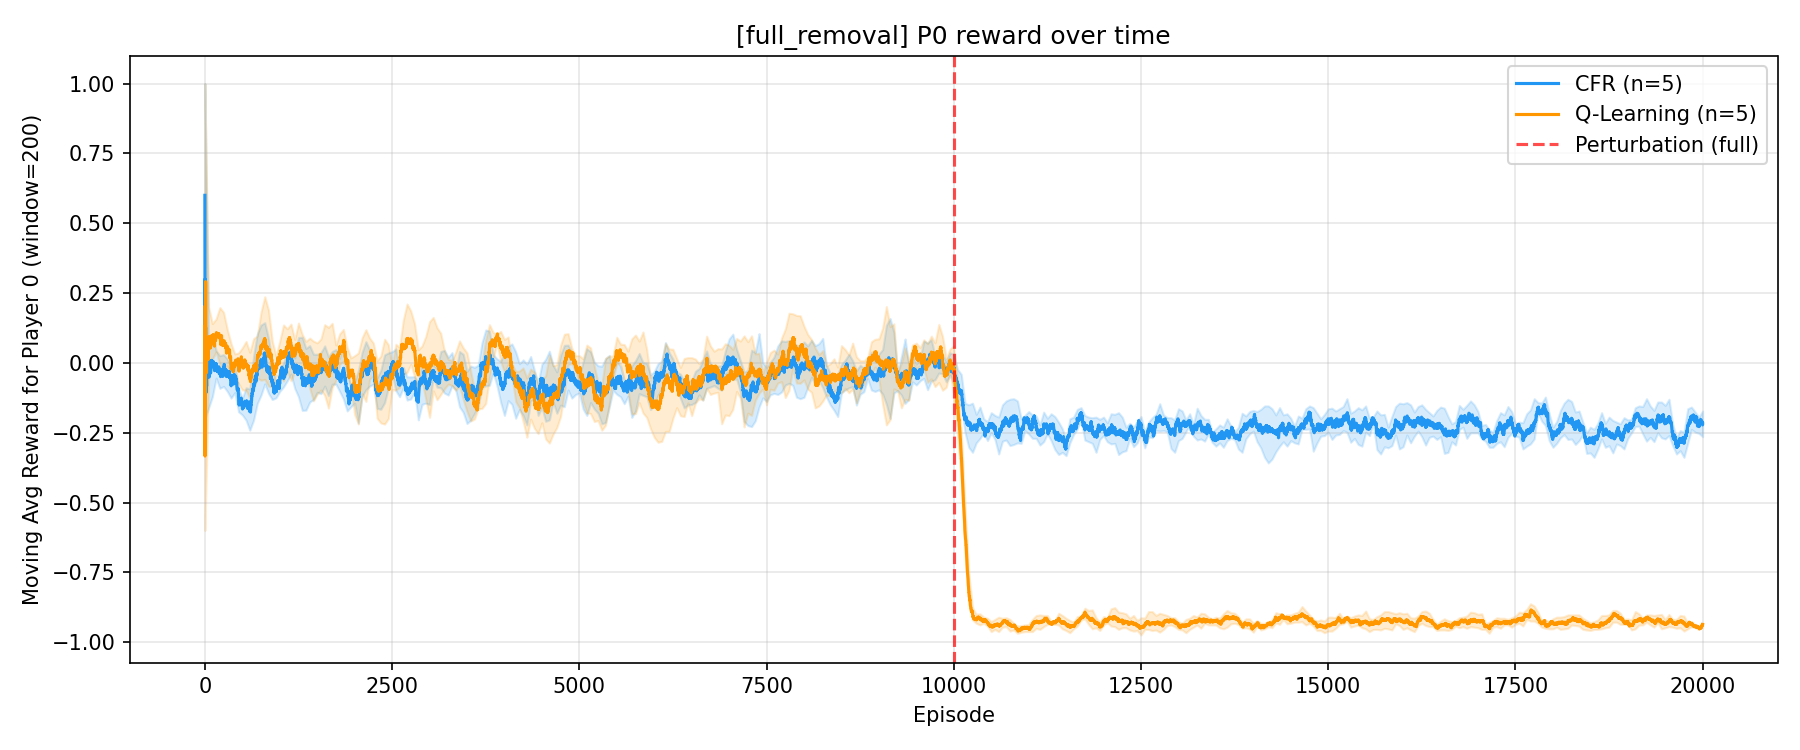
\includegraphics[width=0.85\linewidth]{figures/full_removal.png}
\caption{Kuhn Poker, full removal: moving-average Player~0 reward. Q-Learning collapses within a mean of four episodes after perturbation at episode 10{,}000, illustrating the transition to a deterministic exploitation regime.}
\label{fig:kuhn-full}
\end{figure}

\FloatBarrier
\subsection{Kuhn Poker: Root-Only Removal (Capacity 1)}

Bet is removed from Player~0 only at the root. Player~0 retains the call/fold decision at the ``pb'' node.

\begin{table}[ht!]
\centering
\caption{Kuhn Poker, root-only removal (capacity~1).}
\label{tab:kuhn-root}
\begin{tabular}{lcccc}
\toprule
Agent & Pre (95\% CI) & Post (95\% CI) & $p$ & $d$ \\
\midrule
CFR        & $-0.053$ {\small$[-0.066, -0.041]$} & $-0.061$ {\small$[-0.065, -0.055]$} & $0.27$ & $-0.6$ \\
Q-Learning & $-0.035$ {\small$[-0.046, -0.025]$} & $-0.073$ {\small$[-0.081, -0.064]$} & $0.001$ & $-3.6$ \\
\bottomrule
\end{tabular}
\end{table}

As shown in Table~\ref{tab:kuhn-root}, CFR barely shifts ($p = 0.27$, not significant)---removing an action at an indifference point does not change the equilibrium value. Q-Learning drops modestly ($\Delta = -0.037$) then stabilises: the single remaining decision point forces the opponent to bet honestly, bounding exploitation.

\begin{figure}[ht!]
\centering
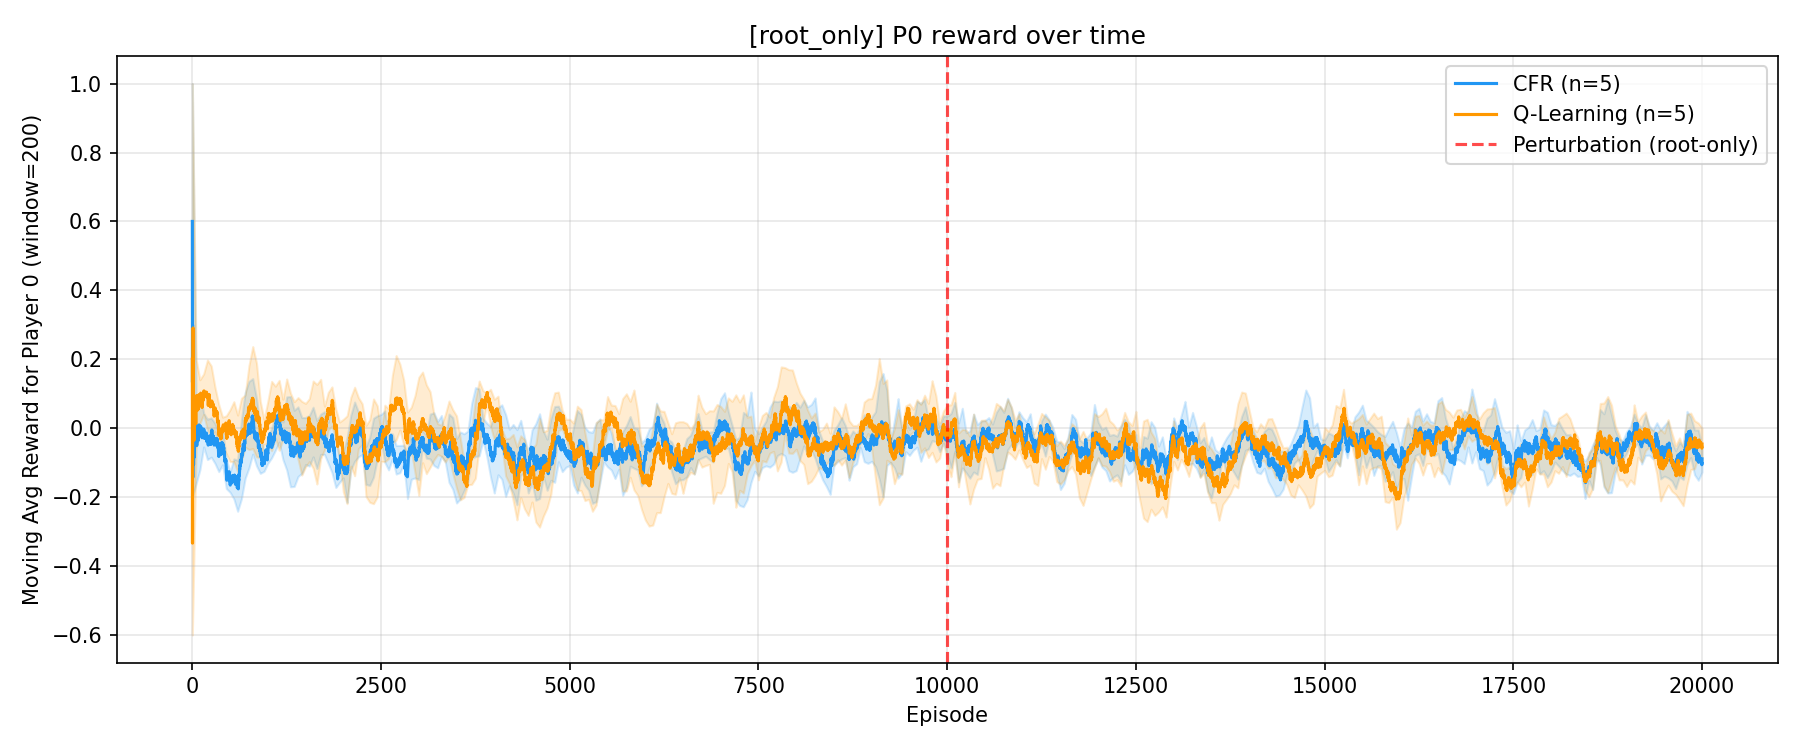
\includegraphics[width=0.85\linewidth]{figures/root_only.png}
\caption{Kuhn Poker, root-only removal: a single retained decision point is sufficient to prevent collapse. Q-Learning stabilises near Nash equilibrium after a brief transient dip.}
\label{fig:kuhn-root}
\end{figure}

\FloatBarrier
\subsection{Decision Capacity Sweep}

\begin{table}[ht!]
\centering
\caption{Kuhn Poker capacity sweep: post-perturbation mean Player~0 reward.}
\label{tab:capacity}
\begin{tabular}{clcc}
\toprule
Capacity & Description & CFR Post & QL Post \\
\midrule
0 & All actions removed             & $-0.231$ & $\mathbf{-0.927}$ \\
1 & Root bet removed, call/fold kept & $-0.061$ & $-0.073$ \\
2 & No perturbation (control)        & $-0.062$ & $-0.034$ \\
\bottomrule
\end{tabular}
\end{table}

As shown in Table~\ref{tab:capacity}, the jump from capacity~0 to capacity~1 is catastrophic ($\Delta = -0.85$ for Q-Learning). The jump from 1 to~2 is marginal ($\Delta = +0.04$). The relationship between decision capacity and exploitability is discontinuous at the zero-to-one boundary---a sharp threshold effect, not a smooth gradient (Figure~\ref{fig:capacity}).

\begin{figure}[ht!]
\centering
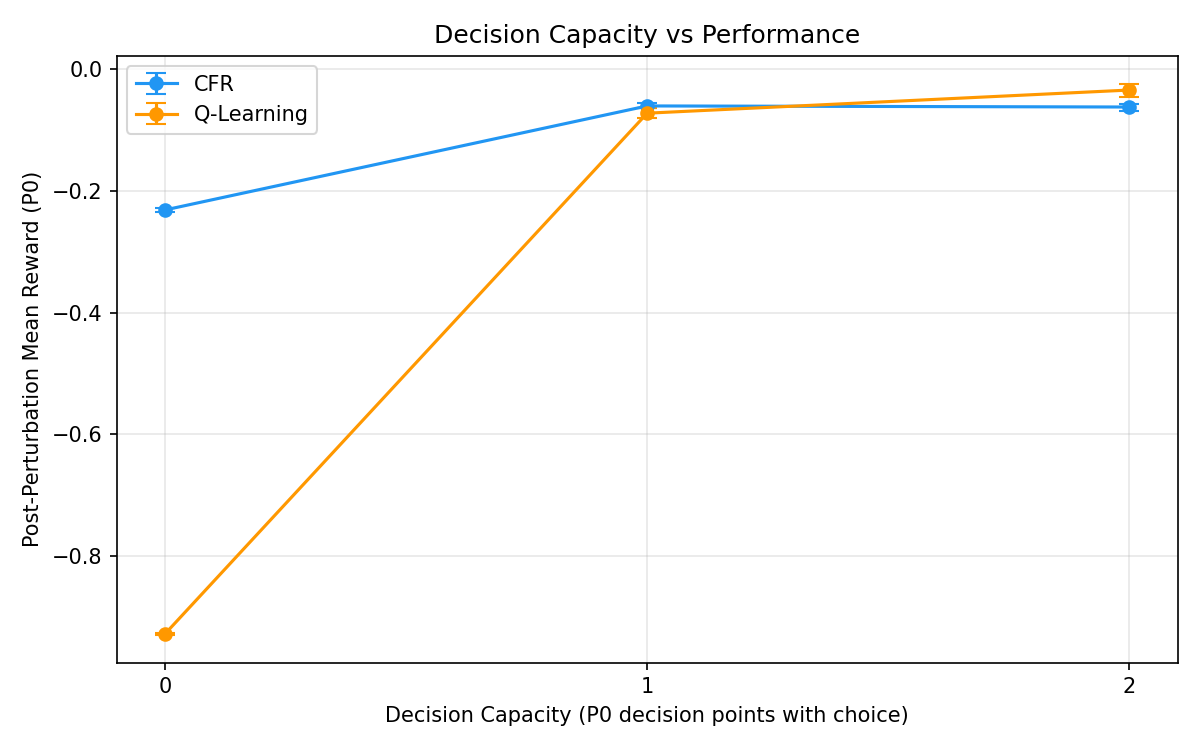
\includegraphics[width=0.7\linewidth]{figures/capacity_sweep.png}
\caption{Decision capacity versus post-perturbation reward with 95\% bootstrap CIs. The discontinuity between capacity~0 and capacity~1 confirms a sharp threshold rather than a gradual decline.}
\label{fig:capacity}
\end{figure}

\FloatBarrier
\subsection{Frozen vs.\ Adaptive Q-Learning}

\begin{table}[ht!]
\centering
\caption{Frozen versus adaptive Q-Learning under full removal (Kuhn).}
\label{tab:frozen}
\begin{tabular}{lcc}
\toprule
Agent & Post (95\% CI) & Collapsed \\
\midrule
CFR        & $-0.231$ {\small$[-0.235, -0.228]$} & 4/5 transient \\
Q-Learning & $\mathbf{-0.927}$ {\small$[-0.929, -0.925]$} & 5/5 (delay: 4 eps) \\
QL-Frozen  & $-0.141$ {\small$[-0.406, -0.007]$} & 2/5 \\
\bottomrule
\end{tabular}
\end{table}

As shown in Table~\ref{tab:frozen}, the paired comparison between Q-Learning and QL-Frozen yields $\Delta = -0.787$, $p = 0.004$, $d = -2.6$. The frozen agent avoids collapse because its policy does not shift toward always-fold. Without the co-adaptation spiral---in which the opponent learns to exploit Player~0's increasing passivity---the perturbation alone causes only moderate degradation.

This isolates continued adaptation under constraint, rather than the quality of the pre-perturbation policy, as the mechanism of collapse. The perturbation creates the vulnerability; self-play learning converts it into exploitation.

\begin{figure}[ht!]
\centering
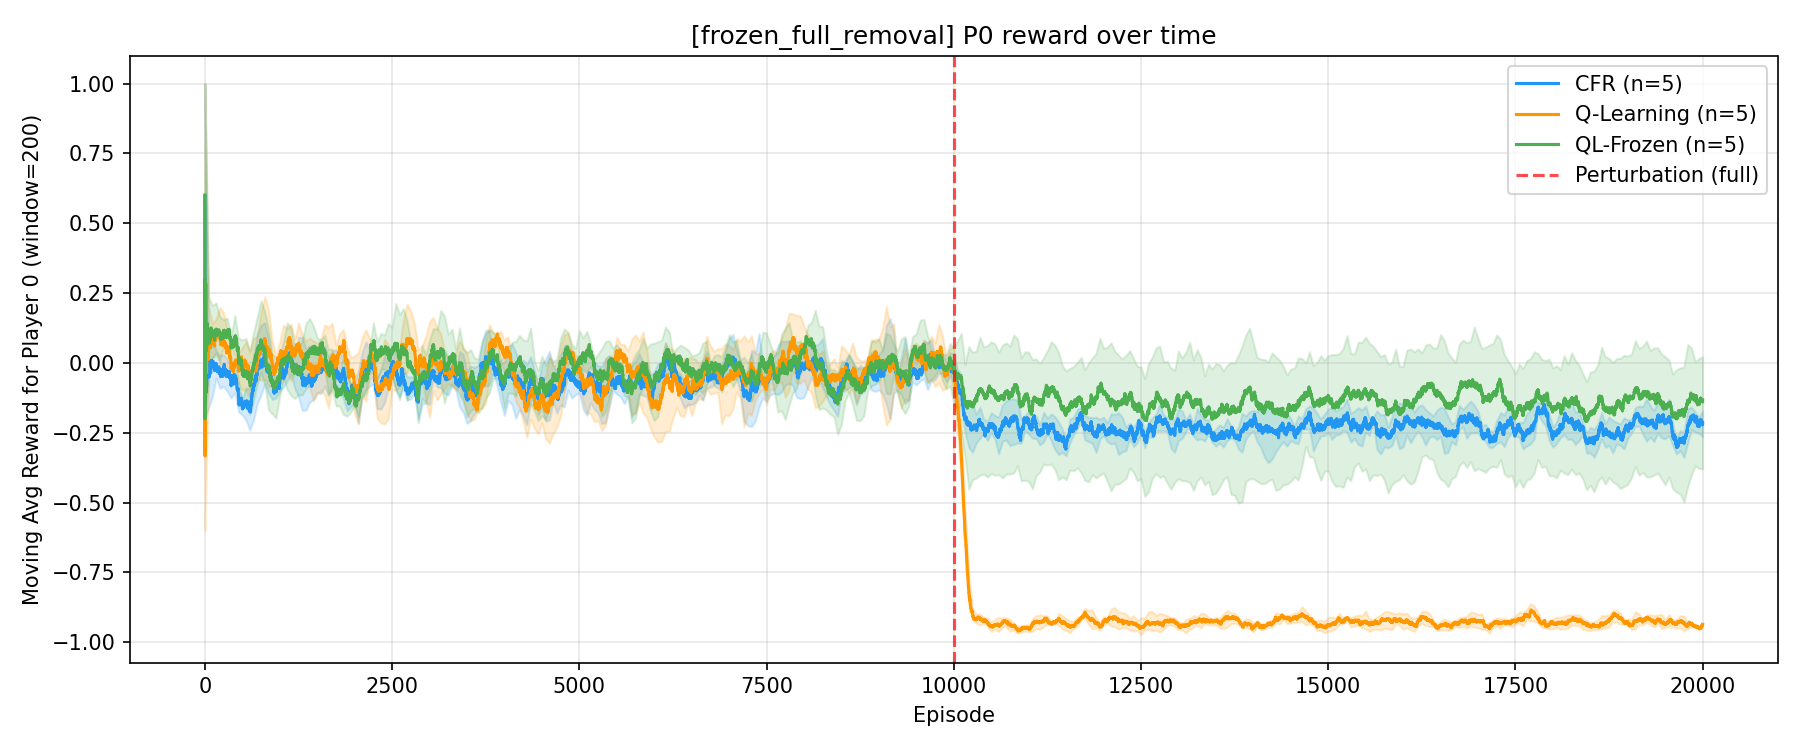
\includegraphics[width=0.85\linewidth]{figures/frozen_full_removal.png}
\caption{Frozen versus adaptive Q-Learning under full removal. QL-Frozen avoids catastrophic collapse, isolating continued co-adaptation---not the perturbation itself---as the mechanism driving exploitation.}
\label{fig:frozen}
\end{figure}

Under root-only removal (capacity~1), no significant difference exists between adaptive and frozen Q-Learning ($p = 0.32$). When capacity $\geq 1$, neither agent collapses regardless of whether learning continues.

\FloatBarrier
\subsection{Perturbation Severity Sweep}

We vary both \emph{when} the perturbation is applied (episode 3{,}000, 10{,}000, or 17{,}000) and \emph{how strongly} (severe: all nodes; mild: root only).

\begin{table}[ht!]
\centering
\caption{Perturbation timing $\times$ severity (Kuhn). Post-perturbation Q-Learning reward.}
\label{tab:severity}
\begin{tabular}{llcc}
\toprule
Timing & Pert.\ Episode & Severe (cap.\ 0) & Mild (cap.\ 1) \\
\midrule
Early & 3{,}000  & $\mathbf{-0.926}$ & $-0.063$ \\
Mid   & 10{,}000 & $\mathbf{-0.927}$ & $-0.073$ \\
Late  & 17{,}000 & $\mathbf{-0.925}$ & $-0.061$ \\
\bottomrule
\end{tabular}
\end{table}

As shown in Table~\ref{tab:severity}, under severe perturbation collapse is \textbf{timing-invariant}: whether Q-values have barely begun learning (early) or are well-converged (late), the outcome is identical. Under mild perturbation, no collapse occurs at any timing. Collapse is structural, not dependent on training stage or convergence level. What determines the outcome is whether the perturbation eliminates all contingent responses, not when it occurs.

\begin{figure}[ht!]
\centering
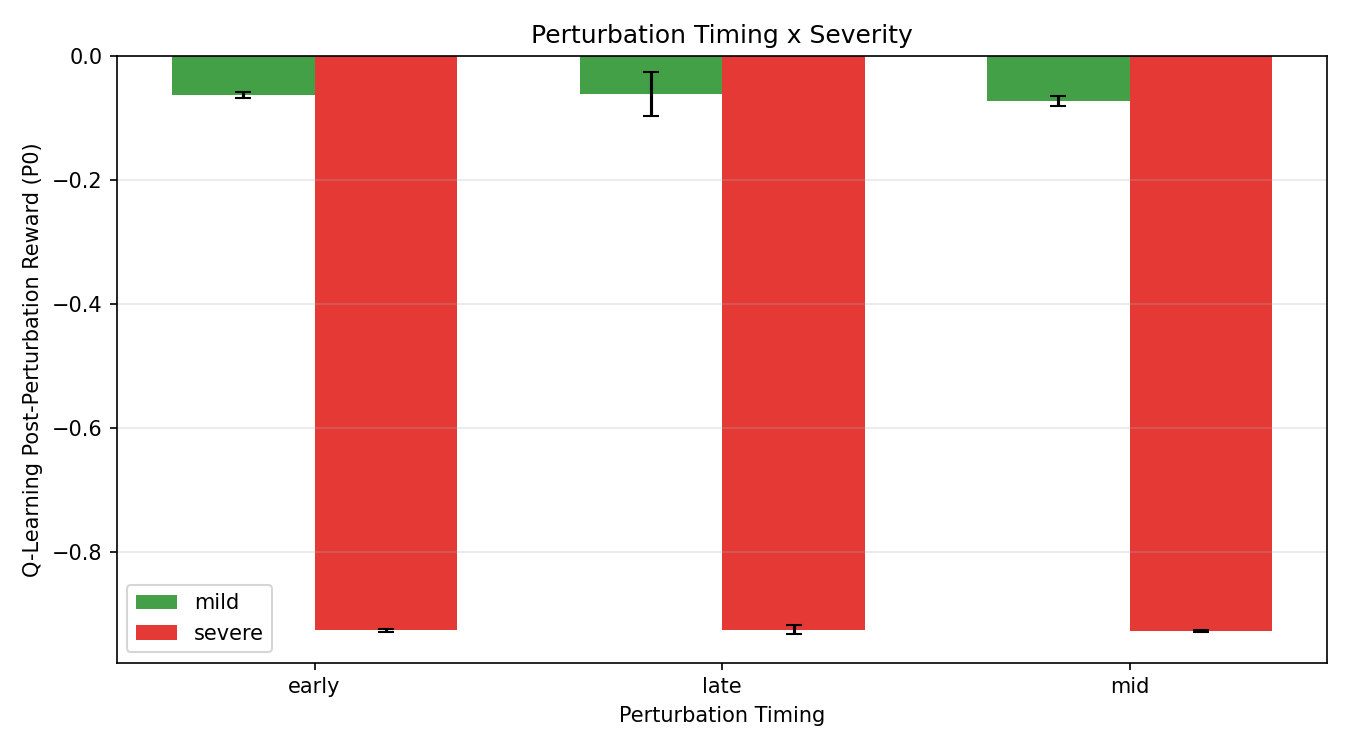
\includegraphics[width=0.75\linewidth]{figures/severity_sweep.png}
\caption{Perturbation timing $\times$ severity. Collapse severity is determined entirely by capacity, not by training stage: severe perturbation produces identical outcomes at all timings.}
\label{fig:severity}
\end{figure}

\FloatBarrier
\subsection{Stochastic Masking}

When the root-only perturbation is applied with 50\% probability per episode (stochastic masking), neither agent collapses: CFR post $= -0.066$ ($p = 0.14$), Q-Learning post $= -0.049$ ($p = 0.06$). Intermittent perturbation does not trigger the exploitation spiral.

\FloatBarrier
\subsection{Leduc Poker: Cross-Game Replication}

\begin{table}[ht!]
\centering
\caption{Leduc Poker, full removal (raise removed at all Player~0 nodes).}
\label{tab:leduc-full}
\begin{tabular}{lcccc}
\toprule
Agent & Pre (95\% CI) & Post (95\% CI) & $p$ & $d$ \\
\midrule
CFR        & $-0.094$ {\small$[-0.111, -0.078]$} & $-0.281$ {\small$[-0.310, -0.247]$} & $0.002$ & $-3.4$ \\
Q-Learning & $-0.122$ {\small$[-0.146, -0.098]$} & $-0.307$ {\small$[-0.429, -0.219]$} & $0.07$  & $-1.1$ \\
\bottomrule
\end{tabular}
\end{table}

Both agents degrade under full removal. Q-Learning's post-perturbation drop is not statistically significant at conventional thresholds ($p = 0.07$), but the direction of the effect is consistent with Kuhn and aligns with the capacity-based explanation. The collapse is less extreme than in Kuhn ($-0.31$ versus $-0.93$) because Leduc retains fold/check-call options even after removing raise, so Player~0 is not completely passive. Collapse speed is slower (mean delay: 104 episodes for Q-Learning) due to the larger state space.

\begin{figure}[ht!]
\centering
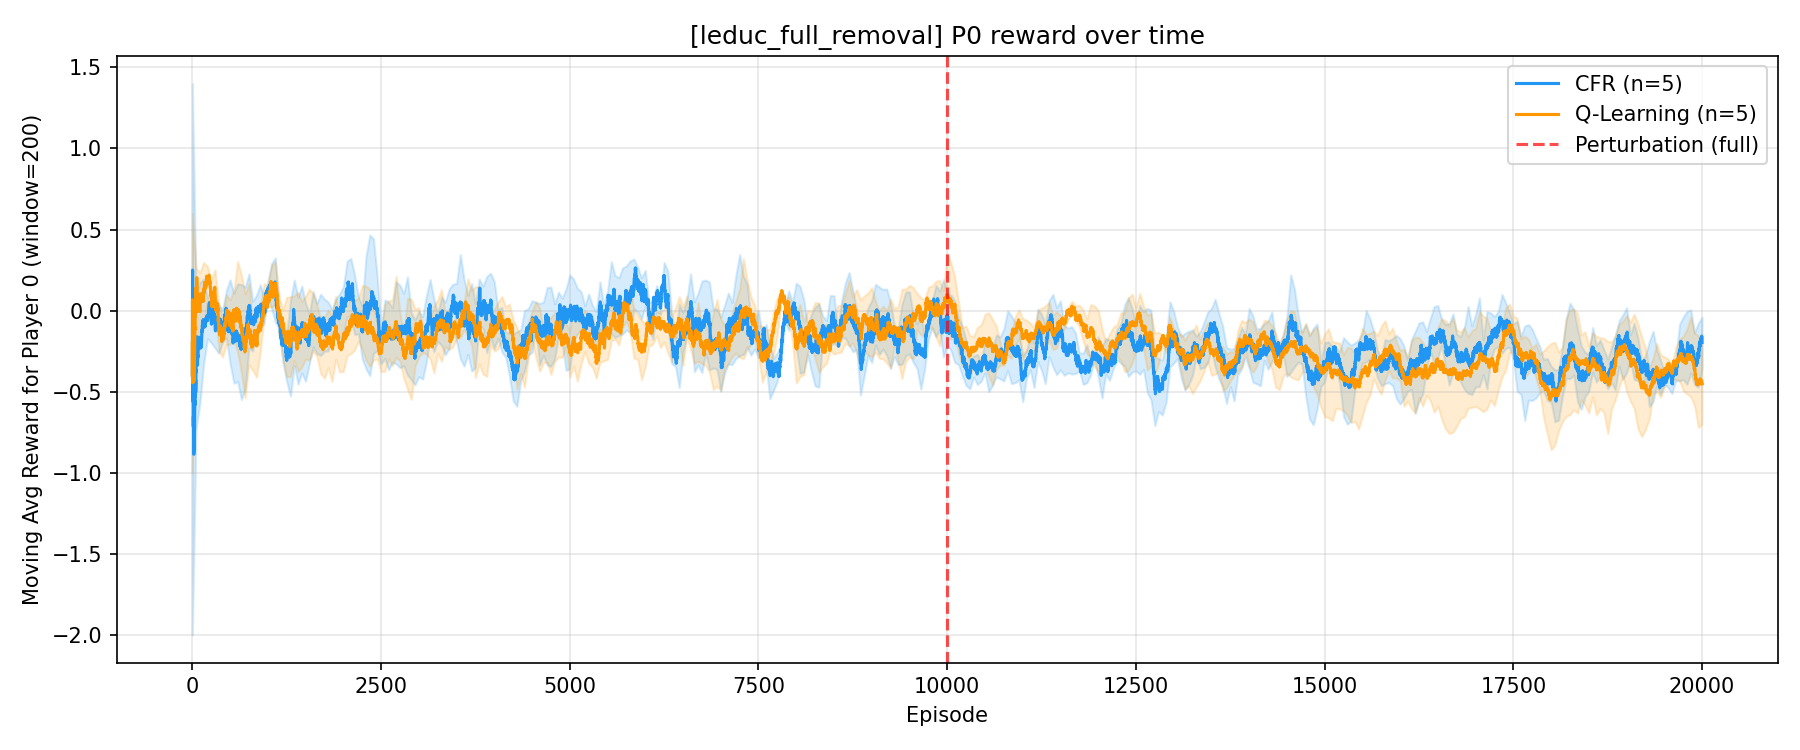
\includegraphics[width=0.85\linewidth]{figures/leduc_full_removal.png}
\caption{Leduc Poker, full removal: both agents degrade after perturbation. Q-Learning shows larger cross-seed variance than in Kuhn, reflecting the greater residual action space in Leduc.}
\label{fig:leduc-full}
\end{figure}

Under root-only removal in Leduc, neither agent degrades significantly (CFR: $p = 0.75$; Q-Learning: $p = 0.40$). The capacity-1 stabilisation observed in Kuhn replicates in Leduc.

\paragraph{Cross-game comparison.}
The qualitative pattern is identical across both games: catastrophic collapse at capacity~0, stability at capacity~$\geq 1$. The quantitative severity scales with residual decision capacity---Leduc retains fold/check-call even under ``full'' raise removal, which partially buffers the collapse.

\begin{table}[ht!]
\centering
\caption{Cross-game comparison of post-perturbation Q-Learning reward.}
\label{tab:cross-game}
\begin{tabular}{lcc}
\toprule
 & Kuhn & Leduc \\
\midrule
Capacity 0 (QL Post)    & $\mathbf{-0.927}$ & $\mathbf{-0.307}$ \\
Capacity 0 (collapse delay) & 4 eps & 104 eps \\
Capacity 1 (QL Post)    & $-0.073$ & $-0.102$ \\
Capacity 1 (collapse?)  & No & No \\
\bottomrule
\end{tabular}
\end{table}

\FloatBarrier
\subsection{Variance Decomposition}

We decompose post-perturbation reward variance into environment (card deals) and policy (action selection) components by fixing one RNG source across seeds (Table~\ref{tab:variance}).

\begin{table}[ht!]
\centering
\caption{Variance decomposition under full removal (Kuhn).}
\label{tab:variance}
\begin{tabular}{lcccc}
\toprule
Agent & $V_\text{total}$ & $V_\text{env}$ & $V_\text{policy}$ & $V_\text{interaction}$ \\
\midrule
CFR        & $2.1 \times 10^{-5}$ & $1.5 \times 10^{-5}$ & $2.8 \times 10^{-5}$ & $-2.2 \times 10^{-5}$ \\
Q-Learning & $5 \times 10^{-6}$   & $7 \times 10^{-6}$   & $6 \times 10^{-6}$   & $-8 \times 10^{-6}$ \\
\bottomrule
\end{tabular}
\end{table}

As shown in Table~\ref{tab:variance}, post-perturbation Q-Learning variance is extremely low across all sources. The near-zero total variance confirms that collapse corresponds to a deterministic fixed point of the self-play dynamics: the opponent converges to the same exploitation strategy regardless of card randomness or exploration noise. This indicates that collapse is not merely instability but convergence to a deterministic attractor under self-play dynamics---a qualitative distinction from the high-variance oscillations typically associated with training failure.

\FloatBarrier
% ===================================================================
\section{Conclusion}

We have shown that a minimal threshold in decision capacity determines whether self-play RL agents catastrophically collapse under asymmetric action-space perturbations. A single remaining contingent response---call/fold in Kuhn, any non-forced action in Leduc---compels the opponent to maintain strategic diversity, bounding losses near Nash equilibrium. When no contingent responses remain, the opponent can enforce a dominant strategy through co-adaptation: the constrained agent's forced passivity removes any incentive for honest play, collapsing the game to deterministic exploitation within episodes.

This threshold is structural. It does not depend on how well-trained the agent is, when the constraint is imposed, or the specific game---only on whether the agent retains at least one genuine decision.

\paragraph{Limitations.}
Our experiments are restricted to small tabular games (Kuhn: 12 information sets; Leduc: 288) with exact CFR solutions and tabular Q-learning. Whether the threshold effect persists under function approximation, larger state spaces, or continuous action spaces remains open. The number of seeds (five) is sufficient for detecting large effects but limits statistical power for subtler comparisons (e.g., Leduc Q-Learning full removal, $p = 0.07$).

\paragraph{Future work.}
Natural extensions include: (i)~scaling to larger games using neural network function approximation; (ii)~studying whether the threshold generalises to non-zero-sum or cooperative settings; (iii)~formalising the connection between decision capacity and exploitability bounds in extensive-form games; and (iv)~investigating whether graduated capacity reduction produces smooth degradation in richer games.

% ===================================================================
\bibliographystyle{plainnat}
\bibliography{references}

\end{document}
